\documentclass[../main]{subfile}
\graphicspath{\subfix{../images}}
\begin{document}

\begin{figure}[bh]
    \centering
    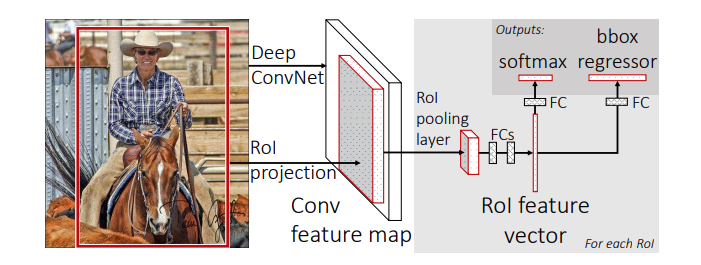
\includegraphics[width=.9\textwidth]{fig1.png}
    \caption{Fast R-CNN结构。一张输入图片和多个感兴趣位置(RoIs)被输入一个全卷积网络。每个RoI被池化为一个固定大小的特征图之后通过全连接层被映射为一个特征向量。网络对每个ROI有两个输出向量:softmax概率和每个类别的边界框回归偏移。整个架构通过多任务损失端到端训练。}
    \label{fig:img1}
\end{figure}

图\ref{fig:img1}阐述了Fast R-CNN的架构。Fast R-CNN网络将一张完整图片和一系列物体候选作为输入。网络首先对图片进行多次卷积和最大池化来产生一个卷积特征图。之后,感兴趣区域(region of interest, \textit{RoI})池化层为每一个物体候选从特征图提取一个固定长度的特征向量。每个特征向量被送入一个最终分为两个兄弟输出层的全连接层序列,一个产生对$K$个物体类加上一个包罗万象的“背景”类的softmax概率估计,另一个则为每一个物体类别输出四个实数值。这四个实数为一个类别编码了调整后的边界框位置。

\subsection{RoI池化层}

RoI池化层使用最大池化来将在任意合法感兴趣区域内的特征转化为一个有着固定空间大小$H\times W$(例如,$7\times 7$)的小特征图,其中$H$和$W$是与RoI无关的层超参数。在这篇文章中,RoI是卷积特征图中的矩形窗口。每个RoI由指定它左上角的$(r, c)$和高宽的$(h, w)$的四元组$(r, c, h, w)$定义。

RoI最大池化通过将$h \times w$的RoI窗口划分为$H \times W$的子窗口网格,其中每个子窗口的大小近似为$h/H \times w/W$,之后对每个子窗口中的值进行最大池化来得到对应网格的输出。正如标准最大池化,每个特征图通道的池化是独立进行的。RoI层是SPPnets\cite{spp}中使用的空间金字塔池化层的特殊情况。我们使用\cite{spp}中给出的池化子窗口计算方式。

\subsection{从预训练的网络初始化}

我们对三种在ImageNet上预训练的网络进行了实验,每一个有五个最大池化层以及五到十三个卷积层(网络细节见4.1节)。当使用预训练网络初始化Fast R-CNN网络时,需要进行三种转化。

第一,最后一个最大池化层被替换为通过设置$H$和$W$来与网络的第一个全连接层兼容的RoI池化层(例如,在VGG16中,$H=W=7$)。

第二,网络的最后一个全连接层和softmax(它们为了1000路ImageNet分类而训练)被替换为早些描述的两个兄弟网络(一个全连接网络和$K+1$类的softmax以及类别特定的边界框回归器)。

第三,网络被修改为接受两个输入数据:一个图片列表和一个这些图片的RoI。

\subsection{为了检测微调}

使用反向传播训练网络所有的参数是Fast R-CNN的一个重要特性。首先,我们来解释为什么SPPnet不能更新空间金字塔池化层下的参数。

根源是当每一个训练样本(也就是RoI)来自不同的图片时,SPP层的反向传播将变得十分低效,而这正是R-CNN和SPPnet的做法。低效源于每个RoI可能有一个非常大的接收域,通常跨越整个输入图像。由于前向传播必须处理全部接收域,所以训练输入是很大的(通常是整个图片)。

我们通过在训练时使用特征共享的优势提出了一个更加高效的训练方法。在Fast R-CNN的训练中,随机梯度下降(SGD)的迷你批是通过层次化采样得到的,首先采样$N$张图片紧接着从每张图片采样$R/N$个RoI。十分重要的是,来自同一张图片的RoI可以在前向和反向传播中共享计算和内存。将$N$变小可以减少迷你批的计算量。例如,当使用$N=2$以及$R=128$时,我们提出的训练方案大约比从128张不同的图片中采样RoI(也就是,R-CNN和SPPnet的策略)快64倍。

对这个策略的一个担忧在于来自同一张图片的RoI是相互关联的,这可能导致训练收敛变慢。然而这个担忧并没有成为实际问题,我们在$N=2$同时$R=128$的情况下获得了很好的结果,并与R-CNN相比进行了更少的SGD迭代。

除了层次化采样,Fast R-CNN使用了一种简化的训练过程,它在单个微调阶段中同时优化softmax分类器和边界框回归器,而不是在三个单独的阶段训练softmax分类器、SVM和回归器\cite{rcnn, spp}。这个过程的组件(损失、迷你批采样策略、通过RoI池化层反向传播和SGD超参数)将会在下面描述。

\paragraph{多任务损失。}Fast R-CNN网络有两个兄弟输出层。第一个输出一个$K+1$个类别上的离散概率分布(为每一个RoI),$p=(p_0,\dots, p_K)$。照常,通过在全连接层的$K+1$个输出上进行softmax得到$p$。第二个兄弟层为每一个类别输出边界框回归偏移,$t^k=(t_x^k, t_y^k, t_w^k, t_h^k)$,其中$k$为类别索引。我们使用\cite{rcnn}中给出的$t^k$参数化方法,其中$t^k$指明了一个与物体候选相关的具有尺度不变性的转化和对数空间的高/宽转化。

我们为每个训练的RoI标记一个ground-truth类别$u$和一个ground-truth边界框回归目标$v$。为了同时训练分类和边界框回归,我们为每个标记的RoI使用一个多任务损失$L$:
\begin{equation} \label{equ:total}
    L(p, u, t^u, v) = L_{cls}(p, u) + \lambda[u\ge1]L_{loc}(t^u, v)
\end{equation}
其中$L_{cls}=-\log p_u$是对于真实类别$u$的对数损失。

第二个任务损失,$L_{loc}$,定义在类别为$u$的真实边界框回归目标元组$v=(v_x, v_y,v_w,v_h)$和类别$u$的预测元组$t^u=(t_x^u, t_y^u, t_w^u, t_h^u)$上。Iverson括号表达式函数$[u \ge 1]$当$u \ge1$时为1否则为0。根据传统,包罗万象的背景类别被标记为$u=0$。对于背景RoI,并不存在ground-truth边界框的表示,所以$L_{loc}$忽略它。对于边界框回归,我们使用损失
\begin{equation} \label{equ:loc}
    L_{loc}(t^u, v) = \sum_{i\in \{x, y,w,h\}}\text{smooth}_{L_1}(t_i^u, v_i),
\end{equation}
其中,
\begin{equation} \label{equ:smooth}
    \text{smooth}_{L_1} = \left\{
    \begin{aligned}
         & 0.5x^2    & \text{if} |x| < 1 \\
         & |x| - 0.5 & \text{otherwise,}
    \end{aligned}
    \right.
\end{equation}
为鲁棒$L_1$损失,相比于R-CNN和SPPnet中使用的$L_2$损失,它对于突出点更加不敏感。对于回归目标无界的情况,使用$L_2$损失训练需要小心地依次调整学习率来避免梯度爆炸。公式\ref{equ:smooth}消除了这个敏感性。

公式\ref{equ:total}中的超参数$\lambda$负责控制两个任务的损失间的平衡。我们\textcolor{violet}{归一化ground-truth回归目标$v_i$的均值为0并为单位方差}。所有的实验使用$\lambda=1$。

我们注意到\cite{6}中使用了一个相关的损失来训练一个不知类别的物体候选网络。与我们的方法不同的是,\cite{6}使用两个网络来分离定位和分类。OverFeat\cite{overfeat},R-CNN\cite{rcnn}和SPPnet\cite{spp}也训练了分类器和边界框定位器,然而这些方法使用分阶段训练,我们在5.1节中表明这对于Fast R-CNN是次优的。

\paragraph{迷你批采样。}在微调过程中,每个SGD迷你批都由随机均匀选择(正如常用的方法,我们实际上遍历数据集的排列)的$N=2$张图片构造。我们使用迷你批的大小为$R=128$,从每张图片采样64个RoI。正如\cite{rcnn}中所说的,我们在与ground-truth的IoU重叠至少为0.5的物体候选挑选25\%的RoI。这些RoI构成了标记为前景类别(也就是,$u \ge 1$)的样例。遵循\cite{spp},剩余的RoI从与ground-truth的最大IoU在$[0.1, 0.5)$区间中的物体候选中采样得到。这些是背景样例并被标注为$u=0$。低阈值0.1发挥难例挖掘的启发作用。在训练中,图片以0.5的概率水平翻转。其余的数据增强并未使用。

\paragraph{通过RoI池化层反向传播。}反向传播指引导数通过RoI池化层。虽然由于前向传播过程独立处理所有图片,扩展到$N>1$是十分直接的,但是为了清晰,我们假设每个迷你批只有一张图片($N=1$)。

假设$x_i \in \mathbb{R}$为RoI池化层的第$i$个激活输入,$y_{rj}$是这一层的第$r$个RoI的第$j$个输出。RoI池化层会计算$y_{rj} = x_{i^*(r, j)}$,其中$i^*(r, j) = \text{argmax}_{i^{'}\in R(r, j)}x_{i^{'}}$。$R(r, j)$是输入中输出单元$y_{rj}$最大池化的子窗口的索引集合。单独的$x_i$可能会为多个不同的输出$y_{rj}$赋值。

RoI池化层的\lstinline{backwards}函数通过遵循argmax转化计算每个输入变量$x_i$对于损失函数的偏导数:
\begin{equation}
    \frac{\partial L}{\partial x_i} = \sum_r \sum_j [i = i^*(r, j)] \frac{\partial L}{\partial y_{rj}}
\end{equation}
用语言描述来说,对于每一个迷你批的RoI $r$以及对于每一个池化输出单元$y_{rj}$,如果$i$是argmax通过最大池化为$y_{rj}$选择的,那么偏导数$\partial L / \partial y_{rj}$将会被累加。在反向传播中,偏导数$\partial L / \partial y_{rj}$已经被RoI池化层之上的层的\lstinline{backwards}函数计算得到了。

\paragraph{SGD超参数。}为了softmax分类和边界框回归的全连接层分别通过0均值0.01和0.001标准差的高斯分布初始化。偏差被设置为0。\textcolor{violet}{所有层使用对于权重为1和对偏差为2的每一层学习率以及一个0.001的全局学习率}。当在VOC07或VOC12上运行时,我们为SGD迷你批迭代30k次,之后降低学习率至0.0001并再迭代10k次。正如后面将要描述的,当在更大的数据集上训练时,我们进行更多次SGD迭代。我们使用了0.9的动量以及0.0005的参数(在权重和偏差上)衰减。

\subsection{尺度不变性}

为了实现尺度不变的物体检测,我们探索了两种方式:(1)通过“蛮力”学习以及(2)通过使用图片金字塔。这些策略遵循了\cite{spp}中的两种方法。在蛮力法中,每张图片在训练和测试中在一个预先定义的像素尺寸上被处理。网络必须直接从训练数据学习尺度不变的物体检测。

多尺度方法,与之形成对比,通过图片金字塔为网络提供了近似的尺度不变性。在测试时,使用图片金字塔来近似尺度归一化每个物体候选。遵循\cite{spp},在多尺度训练中每次图片被采样时,我们随机采样一个金字塔尺寸,作为一种数据增强的形式。由于GPU内存的限制,我们仅在较小的网络上对多尺度训练进行了实验。

\end{document}